\chapter{Projektphase 2 – Webserver}
Die Phase Webserver soll demonstrieren, für welche typischen Angriffsmethoden Webseiten anfällig sind. Dabei werden im Rahmen der Demonstration zwei Angriffe durchgeführt – eine \ac{XSS} Attacke und eine SQL Injection. 
\section{Setup}
\subsection{Datenbank}
Für das Projekt wurde PostgreSQL (auch einfach als Postgres bezeichnet) als Datenbank gewählt. So wurde über Docker eine Container-Instanz einer Postgres Datenbank gestartet, die auf einem Port auf der Hostmaschine auf Nachrichten wartet und über die Adresse localhost:5432 erreichbar ist. \\
Die Datenbank enthält ein Schema "blog", welches die beiden Tabellen – User und Post – beinhaltet. Diese beiden Tabellen besitzen jeweils eine inkrementierende ID als Primärschlüssel. 

\begin{figure}
    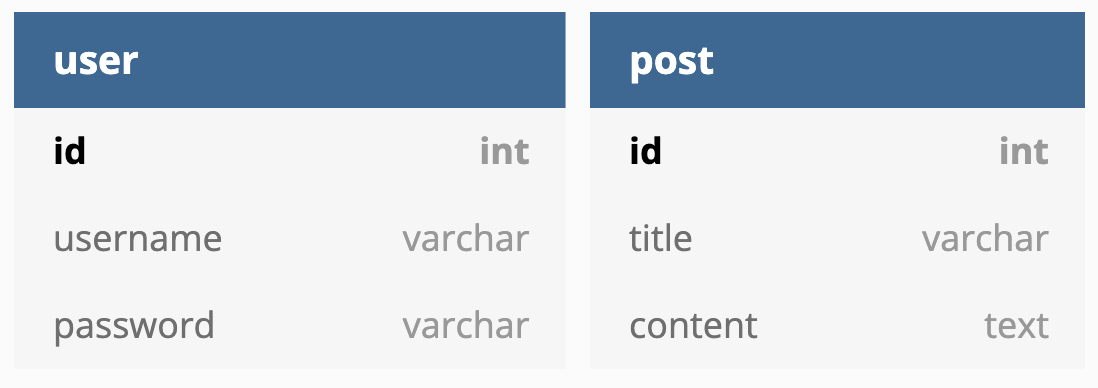
\includegraphics[width=\linewidth]{img/database.png}
    \caption{Database Setup}
    \label{fig:database}
\end{figure}

Die Tabelle User enthält dabei zusätzlich den Benutzernamen und das Passwort des Nutzers – wobei beide bewusst im Klartext gespeichert werden. 
Die Tabelle Post enthält neben der ID noch die Attribute Title und Content, welche bei der Ausgabe der Posts angezeigt werden. 
Als Vorbereitung für die Demonstration beider Attacken wurden bereits Beispiel-Posts und User angelegt, um ein anschaulicheres Ergebnis zu erhalten.
\pagebreak
\subsection{API}

\begin{figure}
    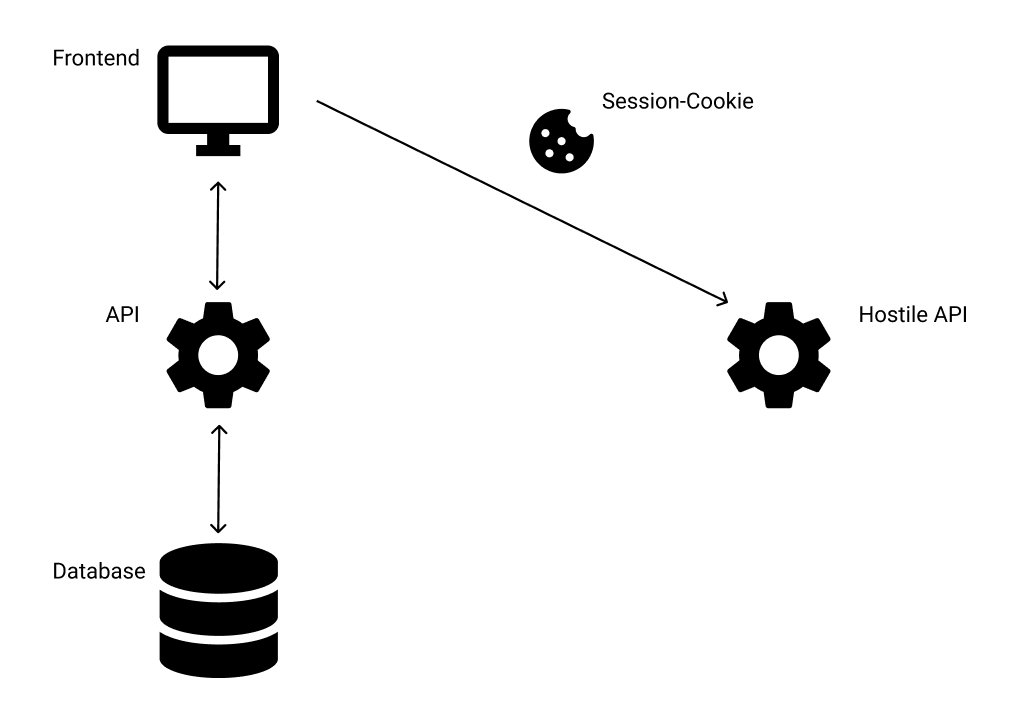
\includegraphics[width=\linewidth]{img/phase2.png}
    \caption{API Setup}
    \label{fig:api}
\end{figure}
Zur Demonstration der beiden Attacken werden zwei APIs genutzt. Beide werden mit Hilfe des Express.js Frameworks implementiert. \\
Die erste – und umfangreichere – API stellt die Schnittstelle zur Datenbank der Blog-Applikation dar. Hier werden die typischen CRUD Operationen durchgeführt und ans Frontend angebunden. Zudem wird die Session-Erstellung hier geregelt.\\
Zu Demonstrationszwecken wurden bewusst Sicherheitsfunktionen in dieser API umgangen. Es wurde zum Beispiel darauf verzichtet, das HTTPOnly Attribut des Cookies zu setzen, was den Zugriff auf den Cookie aus einem Skript heraus verhindern würde. Zudem wird der Cookie im Klartext verschickt, anstatt verschlüsselt zu werden, was ebenfalls die potentielle Sicherheit der Demonstrationsapplikation untergräbt.\\
Die andere API – im Weiteren als bösartige API bezeichnet – stellt den Angreifer dar. Sie verfügt nur über eine einzige Methode, über welche der Session-Cookie des Opfers abgefangen wird. 
\subsection{Frontend}
Das Frontend bildet einen Weblog ab, welcher das Posten von Textbeiträgen ermöglicht. Im Eingabeformular werden vom Besucher Titel und Inhalt eingetragen, bestätigt ("Submit") und über die API an das Backend übermittelt, wo sie in der Datenbank gespeichert werden.\\
Das Frontend wurde mit Vue.js entwickelt und bietet aus diesem Grund einige vordefinierte und standardmäßig aktivierte Sicherheitsfunktionen, die eine \ac{XSS}
 Attacke verhindern sollen. 
\begin{figure}
    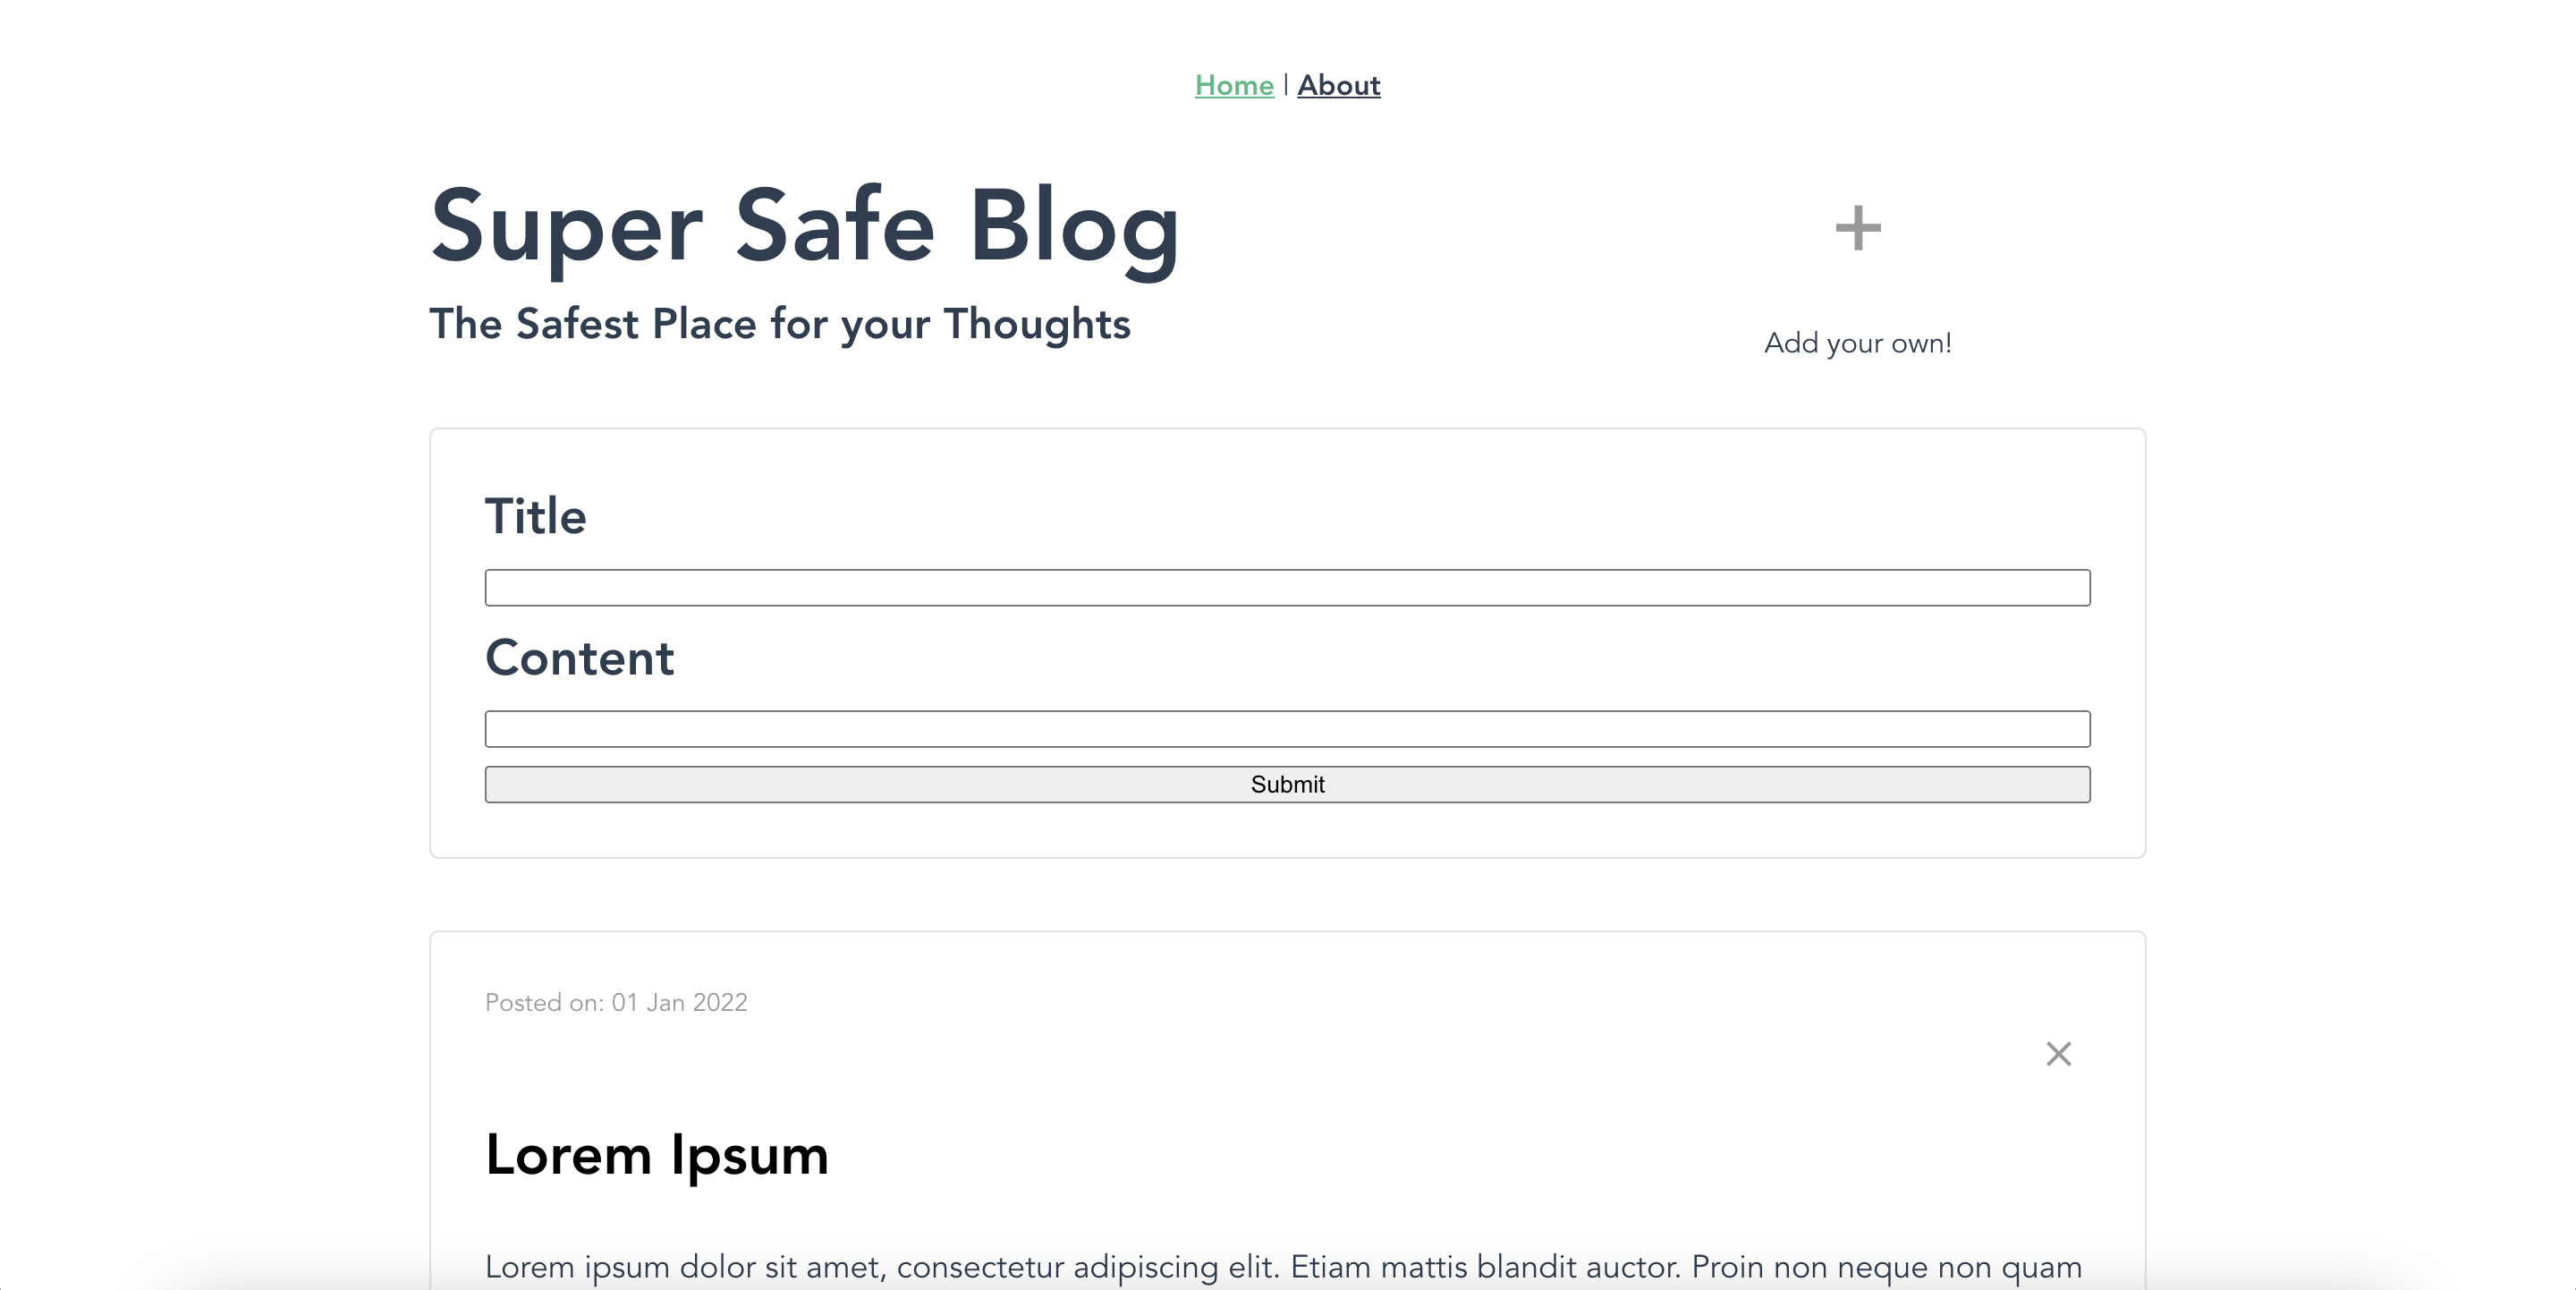
\includegraphics[width=\linewidth]{img/blog.png}
    \caption{Blog-Frontend}
    \label{fig:frontend}
\end{figure}
Um diese Sicherheitsmechanismen zu umgehen, werden die Inhalte aus der Datenbank mit Hilfe des v-HTML Attributs in das Frontend eingebunden, anstatt mit der üblichen ``Mustache`` Notation oder dem v-text Attribut. Diese füllen das innerText Attribut der DOM-Node mit dem gewünschten Inhalt, werden jedoch automatisch ``escaped'', was im Sinne der Sicherheit ist, jedoch gerade die hier beabsichtigte Simulation eines XSS-Angriffes verhindert. . 

\section{Cross-Site-Scripting}

Unter dem Begriff \ac{XSS} versteht man einen Typ der Injektionsattacken, bei dem schadhafter Code – oft in Form eines browserseitigen Scripts – bei einem Endnutzer ausgeführt wird. Diese werden unter anderem durch mangelhafte bzw. fehlende Überprüfung von Nutzereingaben ermöglicht. \\
Um dieses zu demonstrieren, wurde bei diesem Projekt bewusst darauf verzichtet, Nutzereingaben zu überprüfen. 
Das Ziel der Demonstration ist es den Session-Cookie zu stehlen. Um dies zu erreichen wird ein neuer Blog-Post erstellt, bei dem an Stelle eines ``einfachen'' Textes als Inhalt ein schadhaftes HTML <img> Element eingegeben wird. Da es sich bei diesem Element letztlich nur um Text handelt und die Eingabe nicht überprüft wird, wird der Wert in der Datenbank gespeichert. Beim erneuten Aufrufen der Seite versucht der Browser, das <img> Element wie jedes andere auch als Bild zu rendern, erhält jedoch nur einen Fehler, da die im src-Attribut als Bildquelle angegebene URL bewusst fehlerhaft ist. \\
Nun ist es möglich mittels des HTML Attributs ``onerror'' der Applikation vorzuschreiben, wie mit dem Fehler umzugehen ist. Dies wird mittels validem JavaScript Code geschafft. 

    \lstinputlisting{scripts/xss}

Im onerror Attribut wird nun zunächst der Session-Cookie in der Variable cookies gespeichert und dann an die an die Adresse des Angreifers über die bösartige API übermittelt. Sobald der Vorgang abgeschlossen ist wird im Browser-Fenster des Opfers über ein Alert angezeigt, dass das Script funktioniert hat. Abschließend ist der Session-Cookie auf der Console des bösartigen Servers zu finden.

Der Angreifer wäre nun in der Lage diesen Session-Cookie zu nutzen, um sich auf der betroffenen Webseite als ``Opfer'' auszugeben. Demnach könnte der Angreifer die digitale Identität des Opfers stehlen. 
Somit hätte er Zugriff auf die Kontoeinstellungen des Opfers oder er könnte Bestellungen im Namen und mit den Zahlungsmitteln des Opfers tätigen. \\
Große Online-Shops, wie zum Beispiel Amazon, versuchen solche (und ähnliche) Probleme zu verhindern, indem sie vor der Transaktion eine erneute Authentifizierung fordern. So braucht der Angreifer zusätzlich noch Passwort und Benutzername des Opfers, wenn nicht sogar MFA eingerichtet ist.

\section{SQL Injection}
Als zweite Demonstration wird eine SQL Injection durchgeführt. SQL Injections sind eine Art der Injektionsattacken, bei der durch Nutzereingaben valide SQL Queries in die betroffene Applikation injiziert werden. Die OWASP Foundation schreibt dazu: 
\begin{quote}
    A SQL injection attack consists of insertion or “injection” of a SQL query via the input data from the client to the application. A successful SQL injection exploit can read sensitive data from the database, modify database data (Insert/Update/Delete), execute administration operations on the database (such as shutdown the DBMS), recover the content of a given file present on the DBMS file system and in some cases issue commands to the operating system. \cite{abc}
\end{quote}

Das Ziel dieser Demonstration ist es, durch die Eingabe einer bestimmten Zeichenkette einen fremden Post gezielt zu löschen. Dafür wird ein neuer Post eröffnet, bei welchem der Titel frei gewählt, im Content jedoch der folgende String eingegeben wird: 

\lstinputlisting{scripts/injection.sql}

Der String funktioniert, indem zunächst die ursprüngliche Query escaped wird und darauf folgend eine weitere bösartige Query. 
Standardmäßig nutzt die API eine Query, welche mit der Schreibweise ``VALUES ('\$\{Title\}', '\$\{Content\}')' endet, um neue Posts in der Datenbank anzulegen. Wenn nun in der Variable Content die Zeichen '); in Reihenfolge auftreten, werden diese von der Datenbank als Abschluss der Query interpretiert. Daraufhin wird dann eine weitere bösartige Query angehängt, welche von der Datenbank aufgegriffen und verarbeitet wird. Diese Query gibt der Datenbank die Anweisung alle Posts zu löschen, bei denen der Titel ``test'' lautet. 
In einer Produktionsumgebung, wie zum Beispiel die eines Online-Shops, könnte ein derartiger unauthorisierter Eingriff erhebliche Folgen mitsichziehen. So könnte ein bösartiger Akteur sämtliche Inhalte der Datenbank löschen oder publizieren. 
Ähnlich wie die \ac{XSS} Attacken können SQL Injections verhindert werden, indem Nutzereingaben escaped werden.
